% =====================================================================
%  5.2 Arealsetningen — teori og oppgaver
% =====================================================================

\del{1}{Arealsetningen og beviset}

\begin{ordliste}
arealsetningen & Formelen $T = \frac12 ab\sin C$ for arealet av en trekant. & \mittsprak\\
høyde & Det vinkelrette linjestykket fra et hjørne ned til den motstående siden, eller til forlengelsen av den. & \mittsprak\\
spiss vinkel & En vinkel mellom $0^\circ$ og $90^\circ$. & \mittsprak\\
stump vinkel & En vinkel mellom $90^\circ$ og $180^\circ$. & \mittsprak\\
\end{ordliste}

\begin{mustkunne}
\textbf{Arealsetningen.} I trekant $ABC$ står side $a$ overfor vinkel $A$, side $b$ overfor $B$ og side $c$ overfor $C$.
Arealet er
\[ T = \tfrac12\, a\, b \,\sin C \]
Vinkelen $C$ må ligge \emph{mellom} sidene $a$ og $b$. Samme formel gjelder for hvert annet par av sider og vinkelen mellom dem.\par\smallskip
\begin{minipage}[t]{0.48\linewidth}
\centering
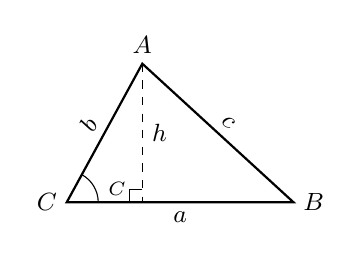
\begin{tikzpicture}[baseline=(current bounding box.north),scale=0.8,font=\small]
  \coordinate (C) at (0,0); \coordinate (B) at (3.6,0);
  \coordinate (A) at (1.2,2.2); \coordinate (D) at (1.2,0);
  \draw[thick] (C)--(B)--(A)--cycle;
  \draw[dashed] (A)--(D);
  \draw (1.0,0)--(1.0,0.2)--(1.2,0.2);
  \draw (0.5,0) arc (0:61.4:0.5);
  \node at (0.8,0.22) {\scriptsize $C$};
  \node[left] at (C) {$C$}; \node[right] at (B) {$B$}; \node[above] at (A) {$A$};
  \path (C) -- (B) node[midway,below,sloped] {$a$};
  \path (C) -- (A) node[midway,above,sloped] {$b$};
  \path (A) -- (B) node[midway,above,sloped] {$c$};
  \path (A) -- (D) node[midway,right] {$h$};
\end{tikzpicture}\par\smallskip
\raggedright
\textbf{Spiss $C$.} Høyden $h$ fra $A$ gir en rettvinklet trekant med hypotenus $b$. Da er $\sin C = \frac{h}{b}$, altså $h = b\sin C$. Grunnlinjen er $a$, så
$T = \frac12 a h = \frac12 ab\sin C$.
\end{minipage}\hfill
\begin{minipage}[t]{0.50\linewidth}
\centering
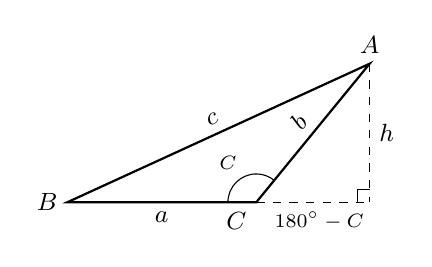
\begin{tikzpicture}[baseline=(current bounding box.north),scale=0.8,font=\small]
  \coordinate (C) at (0,0); \coordinate (B) at (-3.0,0);
  \coordinate (A) at (1.8,2.2); \coordinate (D) at (1.8,0);
  \draw[thick] (C)--(B)--(A)--cycle;
  \draw[dashed] (A)--(D); \draw[dashed] (C)--(D);
  \draw (1.6,0)--(1.6,0.2)--(1.8,0.2);
  \draw (-0.45,0) arc (180:50.7:0.45);
  \node at (-0.45,0.62) {\scriptsize $C$};
  \node[below left] at (C) {$C$}; \node[left] at (B) {$B$}; \node[above] at (A) {$A$};
  \path (B) -- (C) node[midway,below,sloped] {$a$};
  \path (B) -- (A) node[midway,above,sloped] {$c$};
  \path (C) -- (A) node[midway,above,sloped] {$b$};
  \path (A) -- (D) node[midway,right] {$h$};
  \node[below,font=\scriptsize] at (1.0,0) {$180^\circ-C$};
\end{tikzpicture}\par\smallskip
\raggedright
\textbf{Stump $C$.} Høyden faller utenfor trekanten. I den rettvinklede trekanten er vinkelen ved $C$ lik $180^\circ - C$, så $h = b\sin(180^\circ - C) = b\sin C$. Dermed er $T = \frac12 ab\sin C$ også her.
\end{minipage}\par\smallskip
\textbf{Rett vinkel.} Er $C = 90^\circ$, er $\sin C = 1$. Da blir $T = \frac12 ab$: katetene er grunnlinje og høyde. Den kjente formelen er et spesialtilfelle.
\end{mustkunne}

\begin{eksempel}[— areal med $30^\circ$ og $150^\circ$]
En trekant har $a = 6$, $b = 5$ og $C = 30^\circ$. Finn arealet eksakt. Kontroller med $C = 150^\circ$.

\begin{stegtabell}
$T = \frac12 \cdot 6 \cdot 5 \cdot \sin 30^\circ$ & Arealsetningen. $C$ ligger mellom $a$ og $b$.\\
$= 15 \cdot \frac12 = 7{,}5$ & $\sin 30^\circ = \frac12$.\\
$T = \frac12 \cdot 6 \cdot 5 \cdot \sin 150^\circ = 15 \cdot \frac12 = 7{,}5$ & Kontroll: $\sin 150^\circ = \sin(180^\circ - 30^\circ) = \sin 30^\circ$.\\
\end{stegtabell}
Arealet blir det samme, fordi de to vinklene har samme sinus og dermed gir samme høyde.
\end{eksempel}

\begin{vanligfeil}
\begin{itemize}[leftmargin=1.2em,itemsep=1pt,topsep=0pt]
  \item $T = \frac12 ab\sin A$ er feil. Vinkelen må ligge mellom de to sidene: $\frac12 ab\sin C$, $\frac12 bc\sin A$ eller $\frac12 ac\sin B$.
  \item $T = ab\sin C$ er feil. Du glemmer $\frac12$. Rett vinkel gir $T = \frac12 ab$, ikke $ab$.
  \item «Formelen gjelder bare for spisse vinkler» er feil. For stump $C$ er $\sin C = \sin(180^\circ - C)$, og beviset over virker like godt.
\end{itemize}
\end{vanligfeil}

\nivaahode{1}

\oppg{1.1}{1}{\uh}
Finn arealet av trekanten. Svar eksakt.
\begin{tasks}(2)
  \task $a = 4$, $b = 6$ og $C = 30^\circ$
  \task $a = 7$, $b = 4$ og $C = 90^\circ$
  \task $a = 10$, $b = 2$ og $C = 150^\circ$
  \task $a = 8$, $b = 3$ og $C = 45^\circ$
\end{tasks}

\oppg{1.2}{1}{\uh}
Se på figuren.
\begin{minipage}[t]{0.40\linewidth}
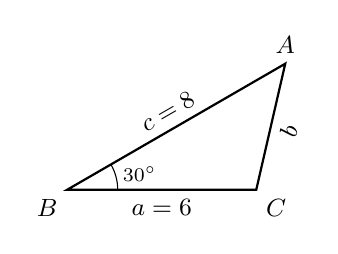
\begin{tikzpicture}[baseline=(current bounding box.north),scale=0.8,font=\small]
  \coordinate (B) at (0,0); \coordinate (C) at (3,0); \coordinate (A) at (3.46,2.0);
  \draw[thick] (B)--(C)--(A)--cycle;
  \draw (0.8,0) arc (0:30:0.8);
  \node at (1.15,0.25) {\scriptsize $30^\circ$};
  \node[below left] at (B) {$B$}; \node[below right] at (C) {$C$}; \node[above] at (A) {$A$};
  \path (B) -- (C) node[midway,below,sloped] {$a = 6$};
  \path (B) -- (A) node[midway,above,sloped] {$c = 8$};
  \path (C) -- (A) node[midway,below,sloped] {$b$};
\end{tikzpicture}
\end{minipage}\hfill
\begin{minipage}[t]{0.56\linewidth}
\begin{tasks}(1)
  \task Hvilken vinkel ligger mellom sidene $a$ og $c$?
  \task Fullfør: $T = \frac12 \cdot \skrivlinje[10mm] \cdot \skrivlinje[10mm] \cdot \sin \skrivlinje[12mm] = \skrivlinje[15mm]$
\end{tasks}
\end{minipage}

\oppg{1.3}{1}{\mh}
Finn arealet. Svar med én desimal.
\begin{tasks}(2)
  \task $a = 7{,}5$ cm, $b = 9{,}2$ cm og $C = 64^\circ$
  \task $a = 12{,}4$ cm, $c = 8{,}6$ cm og $B = 118^\circ$
\end{tasks}

\nivaahode{2}

\oppg{1.4}{2}{\uh}
Finn arealet av trekant $ABC$. Svar eksakt. Avgjør først hvilken vinkel som ligger mellom sidene.
\begin{tasks}(3)
  \task $a = 12$, $b = 9$ og $C = 120^\circ$
  \task $b = 8$, $c = 5$ og $A = 135^\circ$
  \task $a = 10$, $c = 6$ og $B = 60^\circ$
\end{tasks}

\oppg{1.5}{2}{\uh}
I trekant $ABC$ er $a = 6$, $c = 8$ og $B = 120^\circ$. Finn \textbf{den første feilen}. Finn riktig areal.
\[ T = \tfrac12 ac\sin B \;\to\; \tfrac12\cdot 6\cdot 8\cdot\sin 120^\circ \;\to\; 24\cdot\sin 120^\circ \;\to\; 24\cdot\bigl(-\tfrac{\sqrt3}{2}\bigr) \;\to\; -12\sqrt3 \]

\oppg{1.6}{2}{\mh}
Et trekantet seil har to sider på $4{,}2$ m og $3{,}5$ m. Vinkelen mellom dem er $75^\circ$.
\begin{tasks}(1)
  \task Finn arealet av seilet. Svar med én desimal.
  \task Vinkelen endres til $105^\circ$ med de samme sidene. Finn arealet nå. Hva legger du merke til?
\end{tasks}

\oppg{1.7}{2}{\uh}
Trekant $ABC$ har stump vinkel $B$. Høyden $h$ fra $C$ treffer forlengelsen av $AB$ i punktet $D$. Vi skal begrunne at $T = \frac12 ac\sin B$.
\begin{minipage}[t]{0.38\linewidth}
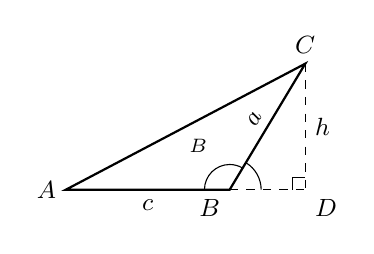
\begin{tikzpicture}[baseline=(current bounding box.north),scale=0.8,font=\small]
  \coordinate (A) at (-2.6,0); \coordinate (B) at (0,0);
  \coordinate (C) at (1.2,2.0); \coordinate (D) at (1.2,0);
  \draw[thick] (A)--(B)--(C)--cycle;
  \draw[dashed] (B)--(D); \draw[dashed] (C)--(D);
  \draw (1.0,0)--(1.0,0.2)--(1.2,0.2);
  \draw (-0.4,0) arc (180:59:0.4);
  \draw (0.5,0) arc (0:59:0.5);
  \node at (-0.5,0.7) {\scriptsize $B$};
  \node[left] at (A) {$A$}; \node[below left] at (B) {$B$}; \node[above] at (C) {$C$}; \node[below right] at (D) {$D$};
  \path (A) -- (B) node[midway,below,sloped] {$c$};
  \path (B) -- (C) node[midway,above,sloped] {$a$};
  \path (C) -- (D) node[midway,right] {$h$};
\end{tikzpicture}
\end{minipage}\hfill
\begin{minipage}[t]{0.58\linewidth}
\begin{tasks}(1)
  \task Skriv vinkel $CBD$ uttrykt ved $B$.
  \task I den rettvinklede trekanten $BCD$ er hypotenusen $a$. Skriv $h$ uttrykt ved $a$ og vinkel $CBD$.
  \task Bruk $\sin(180^\circ - v) = \sin v$ til å skrive $h$ uttrykt ved $a$ og $B$.
  \task Grunnlinjen er $c$. Vis at $T = \frac12 ac\sin B$.
\end{tasks}
\end{minipage}

\nivaahode{3}

\oppg{1.8}{3}{\uh}
Er påstanden alltid, noen ganger eller aldri sann? Begrunn svaret.
\begin{tasks}(1)
  \task To trekanter som begge har sidene $a = 5$ og $b = 8$, har samme areal.
  \task Blir vinkelen $C$ mellom to sider av faste lengder større, blir arealet større.
\end{tasks}

\oppg{1.9}{3}{\uh}
Mia påstår: «Dobler vi vinkelen mellom to sider, dobles arealet.»
Vis med et moteksempel med eksakte verdier at dette ikke gjelder generelt.

\oppg{1.10}{3}{\uh}
En likesidet trekant har side $s$.
\begin{tasks}(1)
  \task Vis at arealet er $T = \dfrac{\sqrt3}{4}s^2$.
  \task Finn $s$ når arealet er $16\sqrt3$.
\end{tasks}

\begin{sjekk}
\begin{tasks}(2)
  \task Finn arealet når $a = 9$, $b = 4$ og $C = 30^\circ$.
  \task Bjørn skriver $T = ab\sin C$. Hva er feil?
  \task! Forklar hvorfor arealsetningen gir $T = \frac12 ab$ når $C = 90^\circ$.
\end{tasks}
\end{sjekk}

% ---------------------------------------------------------------------

\del{2}{Bruke arealsetningen}

\begin{ordliste}
mellomliggende vinkel & Vinkelen mellom to gitte sider. I arealsetningen er det $C$ mellom $a$ og $b$. & \mittsprak\\
to løsninger & Likningen $\sin v = k$ har både en spiss og en stump løsning for $0 < k < 1$. & \mittsprak\\
supplementvinkel & Vinkelen $180^\circ - v$. Den har samme sinus som $v$. & \mittsprak\\
\end{ordliste}

\begin{mustkunne}
\begin{minipage}[t]{0.56\linewidth}
\textbf{Snu formelen.} Når $T$ er kjent, setter vi inn i $T = \frac12 ab\sin C$:
\[ a = \frac{2T}{b\sin C} \qquad \sin C = \frac{2T}{ab} \]
\textbf{Hvorfor to vinkler?} Fordi $\sin(180^\circ - v) = \sin v$, gir både $C = v$ og $C = 180^\circ - v$ samme høyde, og dermed samme areal. Figuren viser begge trekantene.\par\smallskip
\textbf{Hvor mange løsninger?} Er $\sin C$ mellom $0$ og $1$: to vinkler. Er $\sin C = 1$: bare $90^\circ$. Er $\frac{2T}{ab} > 1$: ingen trekant.
\end{minipage}\hfill
\begin{minipage}[t]{0.40\linewidth}
\centering
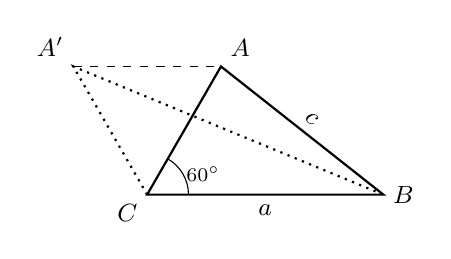
\begin{tikzpicture}[baseline=(current bounding box.north),scale=0.75,font=\small]
  \coordinate (C) at (0,0); \coordinate (B) at (4,0);
  \coordinate (A) at (1.25,2.17); \coordinate (E) at (-1.25,2.17);
  \draw[thick] (C)--(B)--(A)--cycle;
  \draw[thick,dotted] (C)--(E)--(B);
  \draw[dashed] (E)--(A);
  \draw (0.7,0) arc (0:60:0.7);
  \node at (0.95,0.35) {\scriptsize $60^\circ$};
  \node[below left] at (C) {$C$}; \node[right] at (B) {$B$};
  \node[above right] at (A) {$A$}; \node[above left] at (E) {$A'$};
  \path (C) -- (B) node[midway,below,sloped] {$a$};
  \path (A) -- (B) node[midway,above,sloped] {$c$};
\end{tikzpicture}
\end{minipage}
\end{mustkunne}

\begin{eksempel}[1 — finn vinkelen når arealet er kjent]
En trekant har $a = 8$, $b = 5$ og arealet $T = 10\sqrt3$. Finn $C$. Figuren i boksen viser begge mulighetene: $C = 60^\circ$ ($A$) og $C = 120^\circ$ ($A'$).

\begin{stegtabell}
$\frac12 \cdot 8 \cdot 5 \cdot \sin C = 10\sqrt3$ & Arealsetningen med kjent areal.\\
$20\sin C = 10\sqrt3$ & $\frac12 \cdot 8 \cdot 5 = 20$.\\
$\sin C = \frac{\sqrt3}{2}$ & Del begge sider med $20$.\\
$C = 60^\circ$ eller $C = 180^\circ - 60^\circ = 120^\circ$ & Begge vinklene har sinus $\frac{\sqrt3}{2}$.\\
Kontroll: $\frac12 \cdot 8 \cdot 5 \cdot \sin 120^\circ = 20 \cdot \frac{\sqrt3}{2} = 10\sqrt3$ & Begge gir riktig areal.\\
\end{stegtabell}
\end{eksempel}

\begin{eksempel}[2 — areal av en firkant]
I firkant $ABCD$ er diagonalen $AC = 10$ cm, $AB = 8$ cm, $AD = 7$ cm, $\angle BAC = 40^\circ$ og $\angle CAD = 55^\circ$. Finn arealet med én desimal.\par\smallskip
\begin{minipage}[t]{0.32\linewidth}
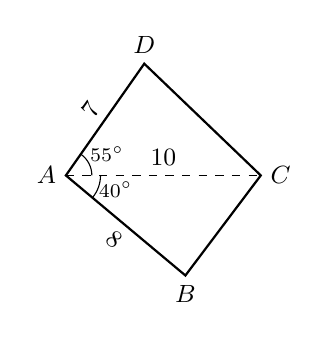
\begin{tikzpicture}[baseline=(current bounding box.north),scale=0.55,font=\small]
  \coordinate (A) at (0,0); \coordinate (C) at (4.5,0);
  \coordinate (B) at (2.76,-2.31); \coordinate (D) at (1.81,2.58);
  \draw[thick] (A)--(B)--(C)--(D)--cycle;
  \draw[dashed] (A)--(C);
  \draw (0.8,0) arc (0:-40:0.8);
  \draw (0.6,0) arc (0:55:0.6);
  \node at (1.15,-0.33) {\scriptsize $40^\circ$};
  \node at (0.95,0.5) {\scriptsize $55^\circ$};
  \node[left] at (A) {$A$}; \node[right] at (C) {$C$};
  \node[below] at (B) {$B$}; \node[above] at (D) {$D$};
  \path (A) -- (B) node[midway,below,sloped] {$8$};
  \path (A) -- (D) node[midway,above,sloped] {$7$};
  \path (A) -- (C) node[midway,above] {$10$};
\end{tikzpicture}
\end{minipage}\hfill
\begin{minipage}[t]{0.64\linewidth}
Diagonalen deler firkanten i trekantene $ABC$ og $ACD$. I begge kjenner vi to sider og vinkelen mellom dem, så vi kan bruke arealsetningen på hver av dem.
\end{minipage}

\begin{stegtabell}
$T_{ABC} = \frac12 \cdot 8 \cdot 10 \cdot \sin 40^\circ \approx 25{,}7$ & Sidene $AB$ og $AC$ med vinkelen $A$ mellom.\\
$T_{ACD} = \frac12 \cdot 10 \cdot 7 \cdot \sin 55^\circ \approx 28{,}7$ & Sidene $AC$ og $AD$ med vinkelen $55^\circ$ mellom.\\
$T = 25{,}7 + 28{,}7 = 54{,}4$ & Legg sammen. Arealet er $54{,}4$ cm$^2$.\\
\end{stegtabell}
\end{eksempel}

\begin{vanligfeil}
\begin{itemize}[leftmargin=1.2em,itemsep=1pt,topsep=0pt]
  \item $\sin C = \frac12$ gir bare $C = 30^\circ$ er feil. Også $C = 150^\circ$ har sinus $\frac12$, og kan gi en trekant med samme areal.
  \item $\sin C = \frac{T}{ab}$ er feil. Det mangler en faktor 2: fra $T = \frac12 ab\sin C$ får vi $\sin C = \frac{2T}{ab}$.
  \item «Det finnes alltid to vinkler» gjelder ikke generelt. Er $\sin C = 1$, finnes bare $90^\circ$. Er $\frac{2T}{ab} > 1$, finnes ingen trekant.
\end{itemize}
\end{vanligfeil}

\nivaahode{1}

\oppg{2.1}{1}{\uh}
Finn siden $a$ når $C$ ligger mellom $a$ og $b$.
\begin{tasks}(3)
  \task $T = 20$, $b = 8$ og $C = 90^\circ$
  \task $T = 12$, $b = 6$ og $C = 30^\circ$
  \task $T = 6\sqrt3$, $b = 4$ og $C = 60^\circ$
\end{tasks}

\oppg{2.2}{1}{\uh}
En trekant har $a = 10$, $b = 4$ og arealet $T = 10$.
\begin{tasks}(1)
  \task Fullfør: $\frac12 \cdot 10 \cdot 4 \cdot \sin C = 10$, så $\skrivlinje[10mm] \cdot \sin C = 10$ og $\sin C = \skrivlinje[12mm]$.
  \task Finn alle vinkler $C$ mellom $0^\circ$ og $180^\circ$ som passer.
\end{tasks}

\oppg{2.3}{1}{\mh}
Finn begge vinklene $v$ mellom $0^\circ$ og $180^\circ$. Svar med én desimal.
\begin{tasks}(3)
  \task $\sin v = 0{,}6$
  \task $\sin v = 0{,}25$
  \task $\sin v = 0{,}9$
\end{tasks}

\nivaahode{2}

\oppg{2.4}{2}{\mh}
En trekant har $a = 9{,}0$, $b = 7{,}0$ og arealet $28$.
\begin{tasks}(1)
  \task Finn begge mulige verdier for vinkelen $C$ mellom $a$ og $b$. Svar med én desimal.
  \task Kontroller den stumpe vinkelen ved å regne ut arealet.
\end{tasks}

\oppg{2.5}{2}{\uh}
Finn alle mulige vinkler $C$ mellom $a$ og $b$. Svar eksakt. Hvis det ikke finnes noen trekant, forklar hvorfor.
\begin{tasks}(1)
  \task $a = 6$, $b = 8$ og $T = 12\sqrt2$
  \task $a = 7$, $b = 4$ og $T = 14$
  \task $a = 6$, $b = 4$ og $T = 15$
\end{tasks}

\oppg{2.6}{2}{\mh}
En firkantet tomt $ABCD$ har diagonalen $AC = 12$ m, $AB = 9$ m, $AD = 8$ m, $\angle BAC = 35^\circ$ og $\angle CAD = 50^\circ$.
Finn arealet av tomten. Svar med én desimal.

\oppg{2.7}{2}{\uh}
En trekant har $a = 6$, $b = 8$ og arealet $12\sqrt3$. Finn $C$. Finn \textbf{den første feilen} og løs riktig.
\[ \tfrac12\cdot 6\cdot 8\cdot\sin C = 12\sqrt3 \;\to\; 24\sin C = 12\sqrt3 \;\to\; \sin C = \tfrac{\sqrt3}{2} \;\to\; C = 60^\circ,\ \text{og det finnes bare én slik trekant} \]

\nivaahode{3}

\oppg{2.8}{3}{\uh}
Lag en trekant $ABC$ med arealet $12$ der vinkelen $C$ mellom sidene $a$ og $b$ er $30^\circ$.
\begin{tasks}(1)
  \task Velg verdier for $a$ og $b$ og vis at arealet blir $12$.
  \task Hvor mange ulike slike trekanter finnes? Begrunn.
  \task Nå er $a = 3$, $b = 8$ og arealet $12$. Hvor mange trekanter finnes da?
\end{tasks}

\oppg{2.9}{3}{\uh}
En trekant har $a = 6$ og $b = 10$, og $C$ ligger mellom dem. Arealet er $T$.
For hvilke verdier av $T$ finnes to, én eller ingen slike trekanter? Begrunn.

\begin{sjekk}
\begin{tasks}(2)
  \task Finn $a$ når $T = 18$, $b = 9$ og $C = 30^\circ$.
  \task Finn begge vinklene $v$ med $\sin v = 0{,}3$. Én desimal.
  \task! Hvorfor gir $v$ og $180^\circ - v$ samme areal når $a$ og $b$ er like?
\end{tasks}
\end{sjekk}
